\section{Introduction}
This homework requires us to implement the Q-Learning algorithm presented in
the paper ``A Q-Learning-Based Topology-Aware Routing Protocol for
Flying Ad Hoc Networks''  by Arafat and Moh.
The paper presents a location-based routing which not only utilizes
the information of single-hop neighbors but also uses the information
of two-hop neighbors (Fig.~\ref{fig:topology}).

\begin{figure}[h]
    \centering
    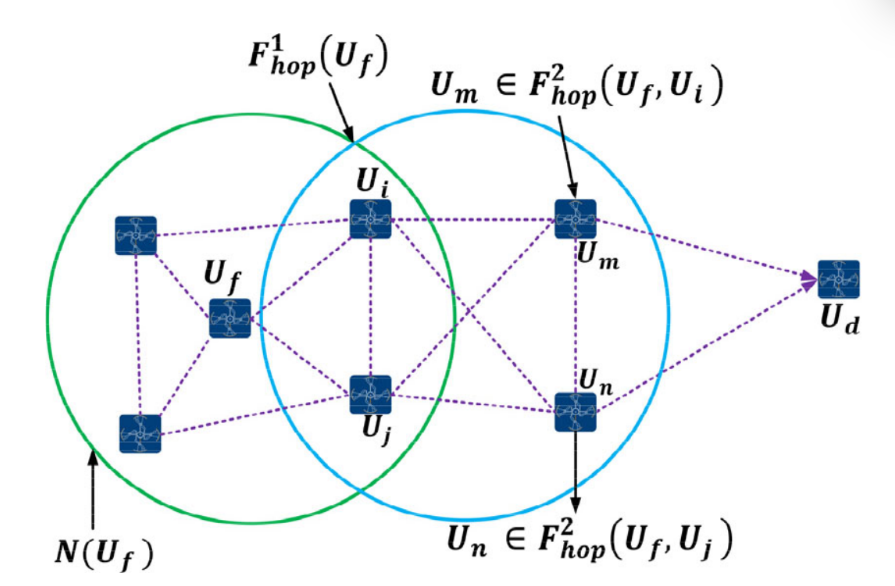
\includegraphics[width=0.5\textwidth]{Figures/paper-fig-6.png}
    \caption{
        The topology of the network.
        $\mathbf{U_f}$ is the drone that is currently forwarding the packet.
        $\mathbf{U_d}$ is the drone that is the destination of the packet.
        $\mathbf{F^1_{hop}(x)}$ is the set of the one-hop neighbors of drone $\mathbf{x}$.
        $\mathbf{F^2_{hop}(x, y)}$ is the set of the two-hop neighbors of drone $\mathbf{x}$ that are one-hop neighbors of drone $\mathbf{y}$.
        The green circle represents the one-hop neighbors of the drone $\mathbf{U_f}$.
        The blue circle represents the two-hop neighbors of the drone $\mathbf{U_f}$ (and the drones in between) that aren't one-hop neighbors of the drone $\mathbf{U_f}$.
    }\label{fig:topology}
\end{figure}

The main contributions given by the given article are:
\begin{itemize}
    \item \textbf{Topology-Aware Routing}: QTAR can operate in highly dynamic environments. For
    topology control, two-hop neighbor information is utilized to estimate the environment and node states. By
    using two-hop neighbor information, we obtain the node
    position, link quality, such as delay, velocity, and residual energy level. The two-hop-based geographic routing
    scheme improves the routing performance and ensures
    successful forwarding from source to destination.
    \item \textbf{Minimazed Communication}: the limited battery power of the dones means that the communication delay must be short. So we change dinamically the hello message interval and the link holding timer to minimize the communication delay basing on the link duration when the topology changes.
    \item \textbf{Loop Free Routing}: two-hop neighbor information minimize the number of hops, thus reducing the probability of loops.
    \item \textbf{Adaptive Q-Learning}: the Q-learning method learns from
    the network environment and allows a quick adaptation.
    \item \textbf{Load Balance}: QTAR doesn't always the shortest path but it takes into account also the residual energy. If a drone is overworked, it will consume more and eventually dying (thus shortening the network lifetime).
\end{itemize}